\documentclass{math}

\usepackage{listings}
\usepackage{pgfplots}
\pgfplotsset{compat=1.8}

\title{Introduction to Cryptography}
\author{Alvin Lin}
\date{January 2018 - May 2018}

\begin{document}

\maketitle

\section*{Introduction to Cryptography Project}

\subsection*{Implementation Details}
This project implements an encryption algorithm based on a family of graphs
using Python. The file \texttt{cipher.py} contains the library code and the
encryption and decryption algorithm. Given a text string and a password, the
functions in \texttt{cipher.py} will encrypt the text string using the password
by turning both into lists of their ASCII code representations and performing
the math described in the project specification. The file \texttt{gui.py}
provides a user friendly GUI interface to the cipher, allowing for a file to
be selected and encrypted.
\par Since we are using a prime modulus of 127 in the algorithm, the character
range that the cipher can handle is limited the ASCII decimal values 0 to 126.
To ensure that all file types can be encrypted by our algorithm, we first run
the file data through base64 to limit the input character set to alphanumerics,
\texttt{+}, \texttt{/}, and \texttt{=}. It is then encrypted and written to the
specified file.
\par Decryption runs the operations in reverse by first decrypting the file
and then decoding it using base64. The raw binary data is then written back to
the output file.

\subsection*{Analysis}

\subsubsection*{Character Frequency Attacks}
To test if the cipher is resistant to character frequency attacks, a large text
file was encrypted and the ciphertext character frequency was compared with
the plaintext character frequency. The plot below shows the average character
distribution using a long text file with passwords of varying length.
\begin{center}
  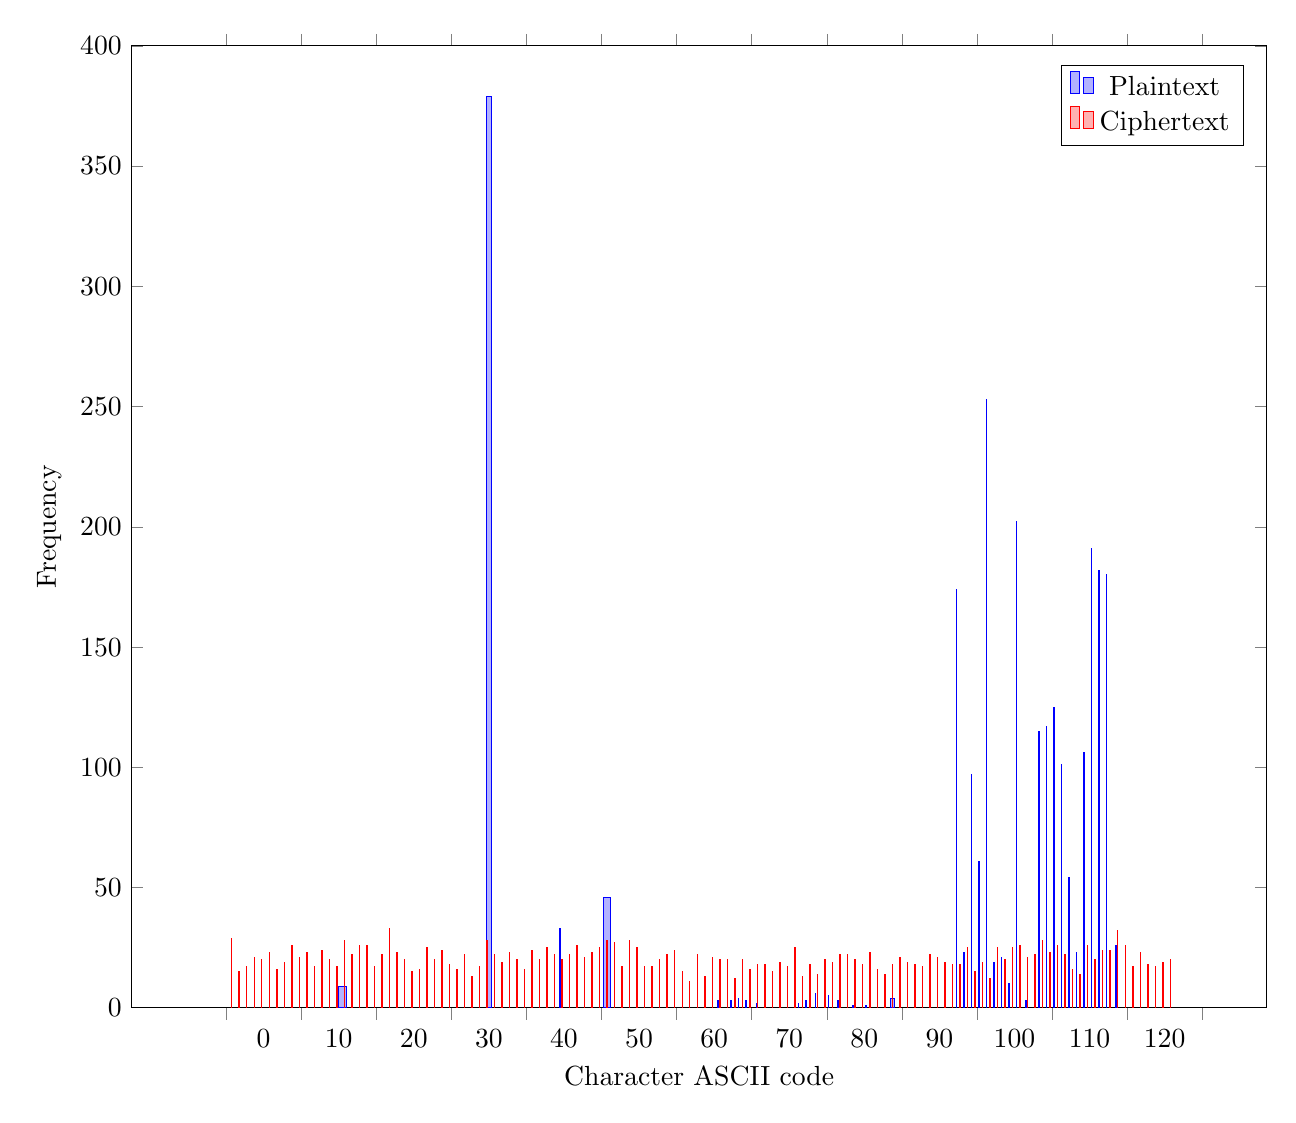
\begin{tikzpicture}
    \begin{axis}[
      ybar interval=0.1, ymax=400, ymin=0, width=16cm, xtick={0,10,...,130},
      xlabel=Character ASCII code, ylabel=Frequency, grid=minor
    ]
      \addplot coordinates { (10, 9) (32, 379) (44, 33) (46, 46) (65, 3) (67, 3) (68, 4) (69, 3) (70, 2) (73, 6) (76, 2) (77, 3) (78, 6) (80, 5) (81, 3) (83, 1) (85, 1) (86, 4) (97, 174) (98, 23) (99, 97) (100, 61) (101, 253) (102, 19) (103, 21) (104, 10) (105, 202) (106, 3) (108, 115) (109, 117) (110, 125) (111, 101) (112, 54) (113, 23) (114, 106) (115, 191) (116, 182) (117, 180) (118, 26) (120, 7) };
      \addlegendentry{Plaintext}
      \addplot coordinates { (0, 29) (1, 15) (2, 17) (3, 21) (4, 20) (5, 23) (6, 16) (7, 19) (8, 26) (9, 21) (10, 23) (11, 17) (12, 24) (13, 20) (14, 17) (15, 28) (16, 22) (17, 26) (18, 26) (19, 17) (20, 22) (21, 33) (22, 23) (23, 20) (24, 15) (25, 16) (26, 25) (27, 20) (28, 24) (29, 18) (30, 16) (31, 22) (32, 13) (33, 17) (34, 28) (35, 22) (36, 19) (37, 23) (38, 20) (39, 16) (40, 24) (41, 20) (42, 25) (43, 22) (44, 20) (45, 22) (46, 26) (47, 21) (48, 23) (49, 25) (50, 28) (51, 27) (52, 17) (53, 28) (54, 25) (55, 17) (56, 17) (57, 20) (58, 22) (59, 24) (60, 15) (61, 11) (62, 22) (63, 13) (64, 21) (65, 20) (66, 20) (67, 12) (68, 20) (69, 16) (70, 18) (71, 18) (72, 15) (73, 19) (74, 17) (75, 25) (76, 13) (77, 18) (78, 14) (79, 20) (80, 19) (81, 22) (82, 22) (83, 20) (84, 18) (85, 23) (86, 16) (87, 14) (88, 18) (89, 21) (90, 19) (91, 18) (92, 17) (93, 22) (94, 21) (95, 19) (96, 18) (97, 18) (98, 25) (99, 15) (100, 19) (101, 12) (102, 25) (103, 20) (104, 25) (105, 26) (106, 21) (107, 22) (108, 28) (109, 23) (110, 26) (111, 22) (112, 16) (113, 14) (114, 26) (115, 20) (116, 24) (117, 24) (118, 32) (119, 26) (120, 17) (121, 23) (122, 18) (123, 17) (124, 19) (125, 20) (126, 14) };
      \addlegendentry{Ciphertext};
    \end{axis}
  \end{tikzpicture}
\end{center}
We can see that there is no correlation between the plaintext and ciphertext's
character frequencies, making this cipher relative resistant to frequency
analysis attacks.

\subsubsection*{Changes in the Plaintext}
Similar plaintexts should yield different ciphertexts even when encrypted with
the same passwords. To test if the cipher is resistant to comparison attacks
based on this idea, we took a known plaintext-ciphertext pair and replaced a
varying segment of the plaintext to compare the shift created in the
ciphertext.
\begin{center}
  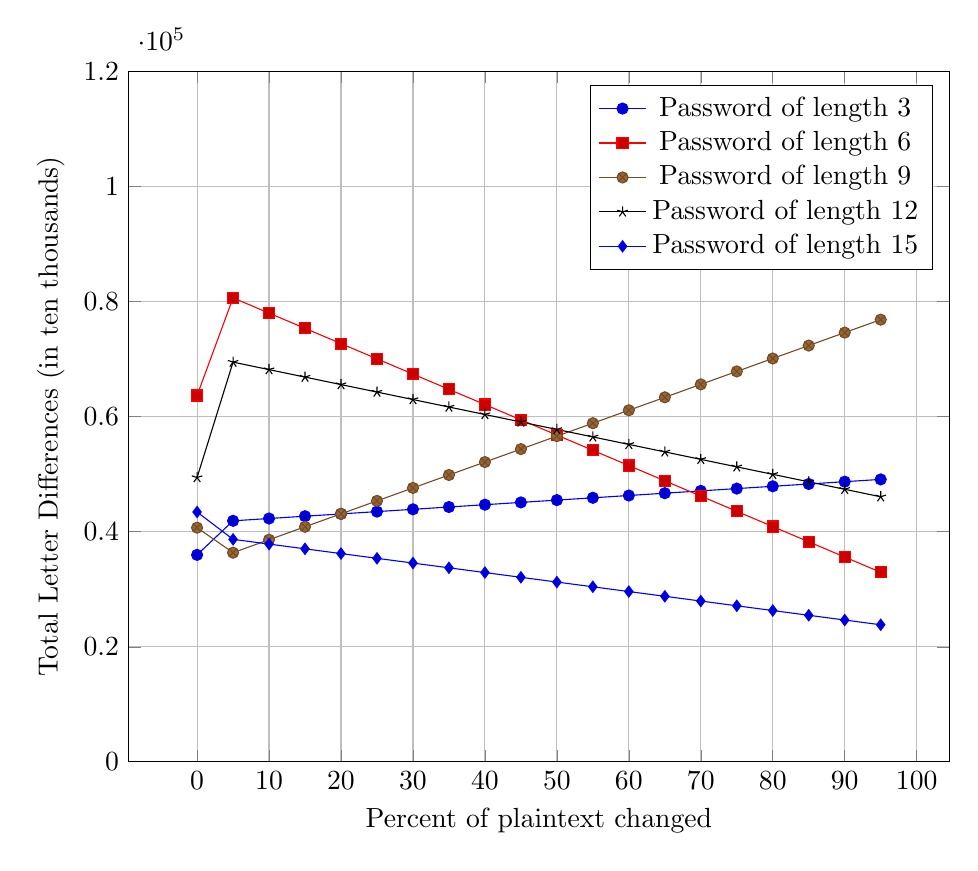
\begin{tikzpicture}
    \begin{axis}[
        grid=major, width=12cm,
        ymin=0, ymax=120000,
        xlabel=Percent of plaintext changed,
        ylabel=Total Letter Differences (in ten thousands)
      ]
      \addplot coordinates { (0, 35984) (5, 41901) (10, 42301) (15, 42701) (20, 43101) (25, 43501) (30, 43901) (35, 44301) (40, 44701) (45, 45101) (50, 45501) (55, 45901) (60, 46301) (65, 46701) (70, 47101) (75, 47501) (80, 47901) (85, 48301) (90, 48701) (95, 49101) };
      \addlegendentry{Password of length 3}
      \addplot coordinates { (0, 63682) (5, 80653) (10, 78003) (15, 75353) (20, 72703) (25, 70053) (30, 67403) (35, 64753) (40, 62103) (45, 59453) (50, 56803) (55, 54153) (60, 51503) (65, 48853) (70, 46203) (75, 43553) (80, 40903) (85, 38253) (90, 35603) (95, 32953) };
      \addlegendentry{Password of length 6}
      \addplot coordinates { (0, 40710) (5, 36365) (10, 38615) (15, 40865) (20, 43115) (25, 45365) (30, 47615) (35, 49865) (40, 52115) (45, 54365) (50, 56615) (55, 58865) (60, 61115) (65, 63365) (70, 65615) (75, 67865) (80, 70115) (85, 72365) (90, 74615) (95, 76865) };
      \addlegendentry{Password of length 9}
      \addplot coordinates { (0, 49425) (5, 69479) (10, 68179) (15, 66879) (20, 65579) (25, 64279) (30, 62979) (35, 61679) (40, 60379) (45, 59079) (50, 57779) (55, 56479) (60, 55179) (65, 53879) (70, 52579) (75, 51279) (80, 49979) (85, 48679) (90, 47379) (95, 46079) };
      \addlegendentry{Password of length 12}
      \addplot coordinates { (0, 43430) (5, 38683) (10, 37858) (15, 37033) (20, 36208) (25, 35383) (30, 34558) (35, 33733) (40, 32908) (45, 32083) (50, 31258) (55, 30433) (60, 29608) (65, 28783) (70, 27958) (75, 27133) (80, 26308) (85, 25483) (90, 24658) (95, 23833) };
      \addlegendentry{Password of length 15}
    \end{axis}
  \end{tikzpicture}
\end{center}

\subsubsection*{Changes in the Password}
Like the previous section, similar passwords should also yield different
ciphertexts when encrypting the same plaintext. To test if our cipher is
resistant to password comparison attacks, we again took a known plaintext but
varied the length of the password to see compare the shift created in the
ciphertext.
\begin{center}
  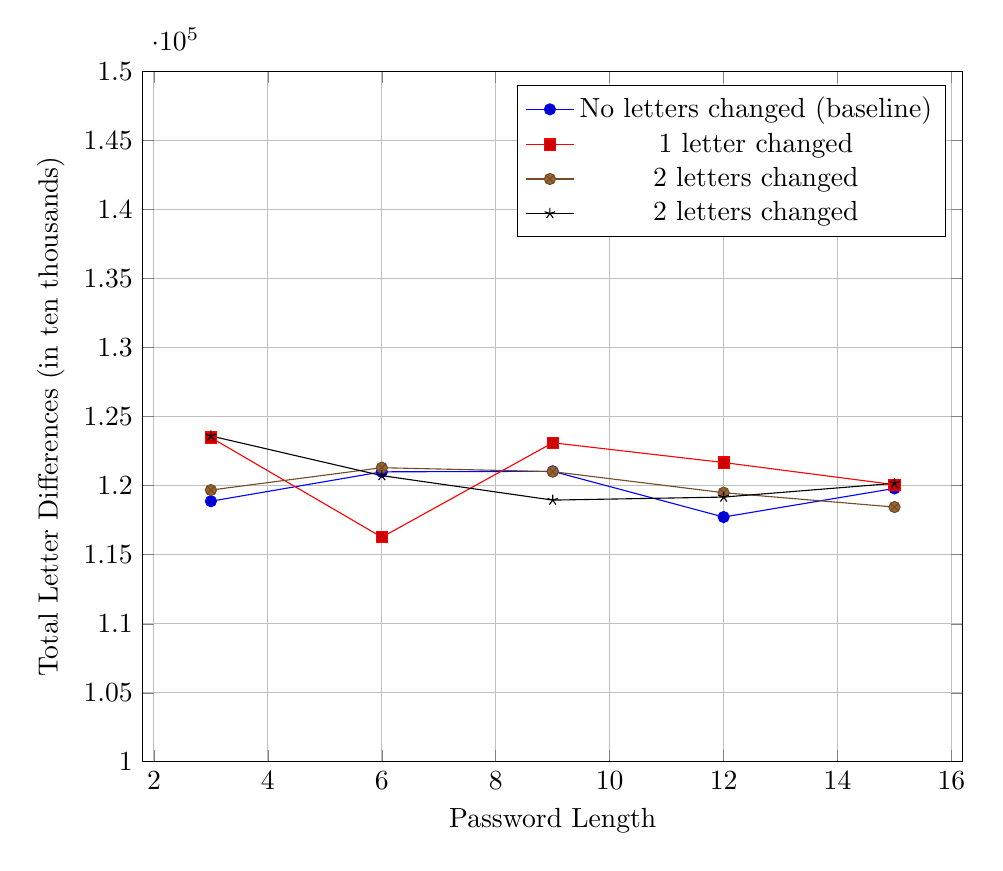
\begin{tikzpicture}
    \begin{axis}[
        grid=major, width=12cm,
        ymin=100000, ymax=150000,
        xlabel=Password Length,
        ylabel=Total Letter Differences (in ten thousands)
      ]
      \addplot coordinates { (3, 118878) (6, 121006) (9, 121044) (12, 117733) (15, 119805) };
      \addlegendentry{No letters changed (baseline)}
      \addplot coordinates { (3, 123486) (6, 116273) (9, 123110) (12, 121680) (15, 120077) };
      \addlegendentry{1 letter changed}
      \addplot coordinates { (3, 119687) (6, 121305) (9, 121021) (12, 119494) (15, 118455) };
      \addlegendentry{2 letters changed}
      \addplot coordinates { (3, 123604) (6, 120731) (9, 118959) (12, 119178) (15, 120172) };
      \addlegendentry{2 letters changed}
    \end{axis}
  \end{tikzpicture}
\end{center}

\end{document}
